\documentclass[11pt,letterpaper]{article}
\usepackage[lmargin=1in,rmargin=1in,tmargin=1in,bmargin=1in]{geometry}
\usepackage{../style/homework}
\usepackage{../style/commands}
\setbool{quotetype}{false} % True: Side; False: Under
\setbool{hideans}{true} % Student: True; Instructor: False

% -------------------
% Content
% -------------------
\begin{document}

\homework{4: Due 01/07}{Sometimes I get so bored I just want to scream, and then sometimes I actually do scream. I just sort of feel out what the situation calls for.}{Kelly Kapoor, The Office}

% Problem 1
\problem{10} Determine if the relations $f(x)$ and $g(x)$ shown below are functions. Explain why or why not. 
	\[
	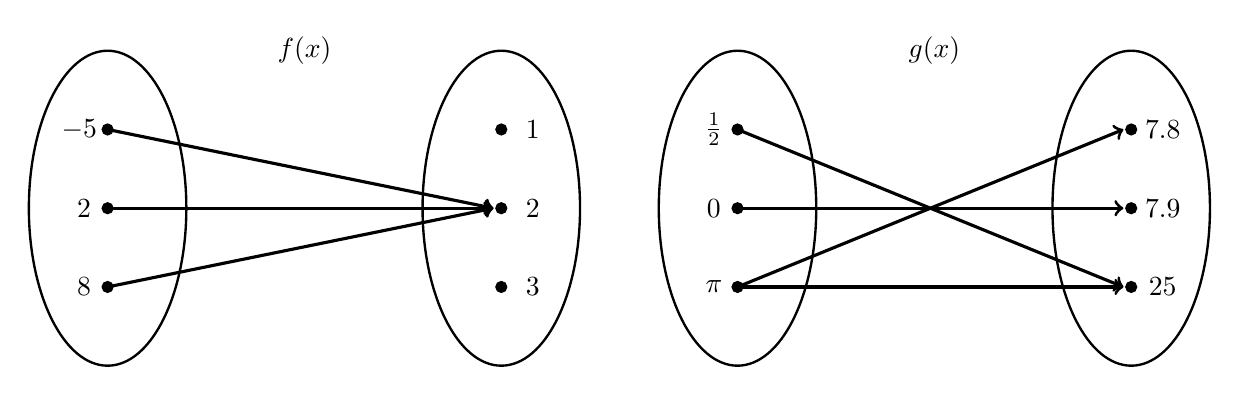
\begin{tikzpicture}
	\node at (2.5,2) {$f(x)$};
	% Ellipses
	\draw[line width=0.03cm] (0,0) circle (1 and 2);
	\draw[line width=0.03cm] (5,0) circle (1 and 2);
	
	% Nodes
	\draw[fill=black] (0,1) circle (0.07);
	\draw[fill=black] (0,0) circle (0.07);
	\draw[fill=black] (0,-1) circle (0.07);
	
	\draw[fill=black] (5,1) circle (0.07);
	\draw[fill=black] (5,0) circle (0.07);
	\draw[fill=black] (5,-1) circle (0.07);
	
	% Arrow
	\draw[line width=0.04cm,->] (0,1) -- (4.9,0);
	\draw[line width=0.04cm,->] (0,0) -- (4.9,0);
	\draw[line width=0.04cm,->] (0,-1) -- (4.9,0);
	
	% Labels
	\node at (-0.3,1) {$\!\!-5$};
	\node at (-0.3,0) {$2$};
	\node at (-0.3,-1) {$8$};
	
	\node at (5.4,1) {$1$};
	\node at (5.4,0) {$2$};
	\node at (5.4,-1) {$3$};
	
	\tikzset{shift={(8,0)}}
	%
	\node at (2.5,2) {$g(x)$};
	% Ellipses
	\draw[line width=0.03cm] (0,0) circle (1 and 2);
	\draw[line width=0.03cm] (5,0) circle (1 and 2);
	
	% Nodes
	\draw[fill=black] (0,1) circle (0.07);
	\draw[fill=black] (0,0) circle (0.07);
	\draw[fill=black] (0,-1) circle (0.07);
	
	\draw[fill=black] (5,1) circle (0.07);
	\draw[fill=black] (5,0) circle (0.07);
	\draw[fill=black] (5,-1) circle (0.07);
	
	% Arrow
	\draw[line width=0.04cm,->] (0,1) -- (4.9,-1);
	\draw[line width=0.04cm,->] (0,0) -- (4.9,0);
	\draw[line width=0.04cm,->] (0,-1) -- (4.9,1);
	\draw[line width=0.04cm,->] (0,-1) -- (4.9,-1);
	
	% Labels
	\node at (-0.3,1) {$\frac{1}{2}$};
	\node at (-0.3,0) {$0$};
	\node at (-0.3,-1) {$\pi$};
	
	\node at (5.4,1) {$7.8$};
	\node at (5.4,0) {$7.9$};
	\node at (5.4,-1) {$25$};
	\end{tikzpicture}
	\] \pspace



\newpage



% Problem 2
\problem{10} Determine if the relations $f(x)$ and $g(x)$ shown below are functions. Explain why or why not. 
	\begin{table}[!ht]
	\centering
	\begin{tabular}{c|rcc|r}
	$x$ & $f(x)$ & \hspace{1cm} & $x$ & $g(x)$ \\ \cline{1-2} \cline{4-5}
	$1$ & $5$ & & $1$ & $6$ \\
	$2$ & $5$ & & $2$ & $8$ \\
	$3$ & $6$ & & $3$ & $10$ \\
	$4$ & $6$ & & $4$ & $12$ \\
	$5$ & $10$ & & $1$ & $13$
	\end{tabular}
	\end{table} \pspace



\newpage



% Problem 
\problem{10} Determine if the relation below is a function or not. If it is a function, explain why. If it is not a function, explain why. 
	\[
	\fbox{
	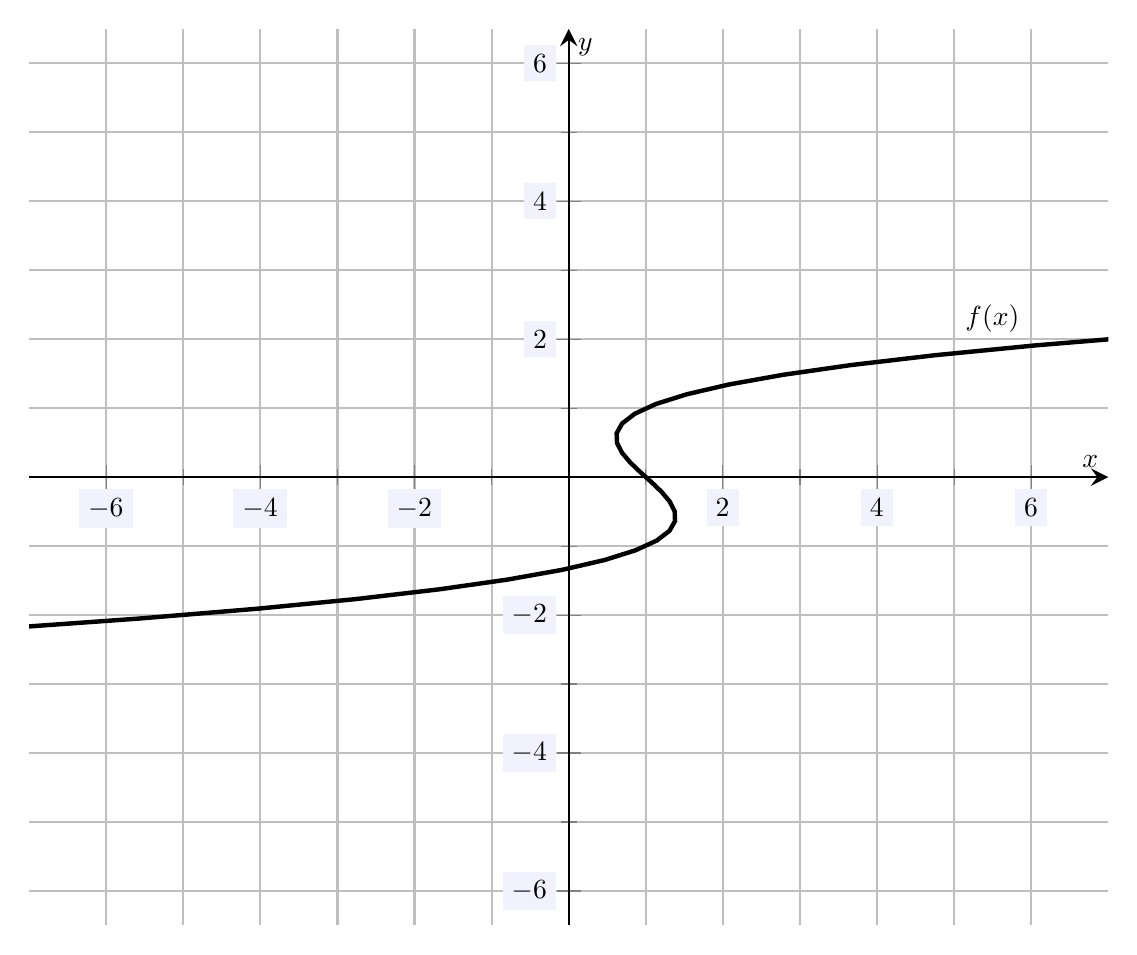
\begin{tikzpicture}[scale=2,every node/.style={scale=0.5}]
	\begin{axis}[
	grid=both,
	axis lines=middle,
	ticklabel style={fill=blue!5!white},
	xmin= -7, xmax=7,
	ymin= -6.5, ymax=6.5,
	xtick={-6,-4,-2,0,2,4,6},
	ytick={-6,-4,-2,0,2,4,6},
	minor tick = {-5,-3,...,5},
	xlabel=\(x\),ylabel=\(y\),
	]
	\node at (5.5,2.3) {$f(x)$};
	\addplot[thick, domain= -7:7, samples=100] ({x^3-x+1},{x});
	\end{axis}
	\end{tikzpicture}
	}
	\]



\newpage



% Problem 3
\problem{10} Determine if the relations $f(x)$ and $g(x)$ shown below are functions. Explain why or why not. 
	\[
	\begin{aligned}
	f(x)&= 6.73 - 13.54x \\[0.3cm]
	g(x)&= \dfrac{6x - 5}{3x^2 + 1}
	\end{aligned}
	\] \pspace



\newpage




% Problem 
\problem{10} Suppose $f(x)$ is the function given below.
	\[
	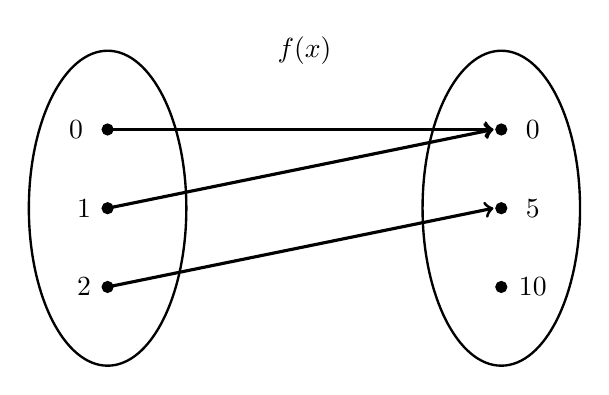
\begin{tikzpicture}
	\node at (2.5,2) {$f(x)$};
	% Ellipses
	\draw[line width=0.03cm] (0,0) circle (1 and 2);
	\draw[line width=0.03cm] (5,0) circle (1 and 2);
	
	% Nodes
	\draw[fill=black] (0,1) circle (0.07);
	\draw[fill=black] (0,0) circle (0.07);
	\draw[fill=black] (0,-1) circle (0.07);
	
	\draw[fill=black] (5,1) circle (0.07);
	\draw[fill=black] (5,0) circle (0.07);
	\draw[fill=black] (5,-1) circle (0.07);
	
	% Arrow
	\draw[line width=0.04cm,->] (0,1) -- (4.9,1);
	\draw[line width=0.04cm,->] (0,0) -- (4.9,1);
	\draw[line width=0.04cm,->] (0,-1) -- (4.9,0);
	
	% Labels
	\node at (-0.4,1) {$0$};
	\node at (-0.3,0) {$1$};
	\node at (-0.3,-1) {$2$};
	
	\node at (5.4,1) {$0$};
	\node at (5.4,0) {$5$};
	\node at (5.4,-1) {$10$};
	\end{tikzpicture}
	\]

\begin{enumerate}[(a)]
\item What is the domain of $f(x)$?
\item What is the codomain of $f(x)$?
\item What is the range of $f(x)$?
\end{enumerate} \pspace



\newpage



% Problem 
\problem{10} Determine whether the point $(2, -1)$ is on the graph of $f(x)= 2x^2 - 5x + 3$. Determine also whether the point $(1, 0)$ is on the graph of $f(x)$. For each, explain why or why not. \pspace



\newpage



% Problem 
\problem{10} Suppose $f(x)$ and $g(x)$ are the functions given below. 
        \begin{table}[!ht]
        \centering
        \begin{tabular}{| c || c | c | c | c | c | c | c |} \hline
	$x$ & $-3$ & $-2$ & $-1$ & $\phantom{-}0$ & $\phantom{-}1$ & $\phantom{-}2$ & $\phantom{-}3$ \\ \hline
	$f(x)$ & $3$ & $-2$ & $1$ & $6$ & $4$ & $-7$ & $0$ \\ \hline
	$g(x)$ & $2$ & $1$ & $0$ & $3$ & $-5$ & $-5$ & $-4$ \\ \hline
	$h(x)$ & $0$ & $1$ & $0$ & $3$ & $0$ & $-1$ & $6$ \\ \hline
        \end{tabular}
        \end{table}

Compute the following: \pspace
        \begin{enumerate}[(a)]
        \item $(f + g)(1)=$ \vfill
        \item $(f - g)(-2)=$ \vfill
        \item $(-2h)(3)=$ \vfill
        \item $\left(\dfrac{h}{g}\right)(0)=$ \vfill
        \item $f(0)\, h(-2)=$ \vfill
        \item $f(2 - h(0))=$ \vfill
        \item $(f \circ g)(0)=$ \vfill
        \item $(g \circ h)(2)=$ \vfill
        \item $(f \circ g \circ h)(1)=$ \vfill
        \item $(h \circ g)(-2)=$
        \end{enumerate} \pspace



\newpage



% Problem 
\problem{10} Suppose $f(x)$ and $g(x)$ are the functions given below. 
	\[
	\begin{aligned}
	f(x)&= 4 - 3x \\[0.3cm]
	g(x)&= x^2 - x + 4
	\end{aligned}
	\]

Compute the following: \pspace
\begin{enumerate}[(a)]
\item $f(2)=$ \vfill
\item $g(1)=$ \vfill
\item $3f(1) - g(2)=$ \vfill
\item $f(x) - g(x)=$ \vfill
\item $f(x) \, g(x)=$ \vfill
\item $\left( \dfrac{f}{g} \right)(x)=$ \vfill
\item $(f \circ g)(0)=$ \vfill
\item $(g \circ f)(1)=$ \vfill
\item $(f \circ g)(x)=$ \vfill
\item $(g \circ f)(x)=$ \vfill
\end{enumerate} \pspace



\newpage



% Problem 
\problem{10} Given the graph of $f(x)$ below, determine whether $f(x)$ has an inverse function. Explain why or why not. 
	\[
	\fbox{
	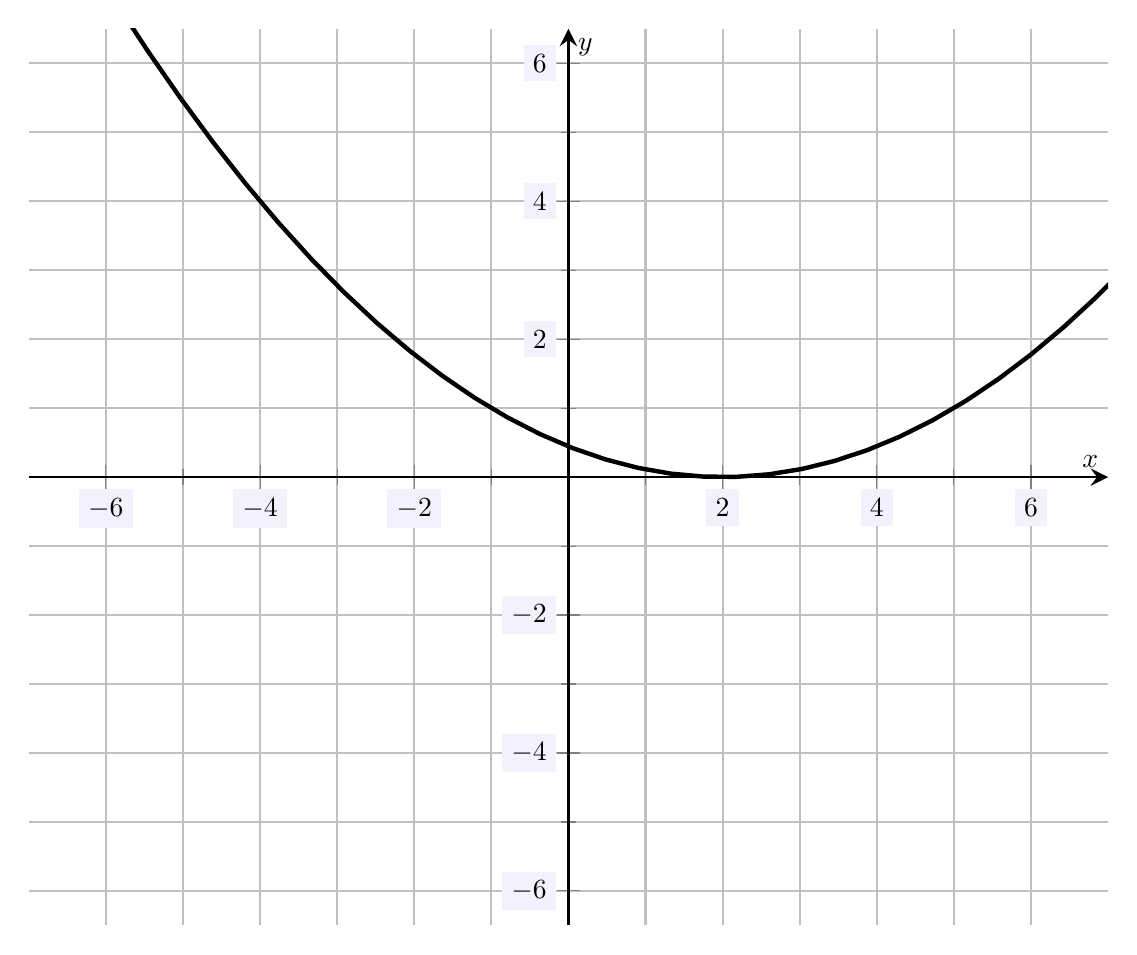
\begin{tikzpicture}[scale=2,every node/.style={scale=0.5}]
	\begin{axis}[
	grid=both,
	axis lines=middle,
	ticklabel style={fill=blue!5!white},
	xmin= -7, xmax=7,
	ymin= -6.5, ymax=6.5,
	xtick={-6,-4,-2,0,2,4,6},
	ytick={-6,-4,-2,0,2,4,6},
	minor tick = {-5,-3,...,5},
	xlabel=\(x\),ylabel=\(y\),
	]
	\addplot[thick, domain= -7:7,samples=100] ({3*x-1},{x^2-2*x+1});
	\end{axis}
	\end{tikzpicture}
	}
	\] \pspace



\newpage



% Problem 
\problem{10} Given the graph of $f(x)$, sketch the function $f^{-1}(x)$. Determine also $f^{-1}(1)$ and $f^{-1}(2)$. 
	\[
	\fbox{
	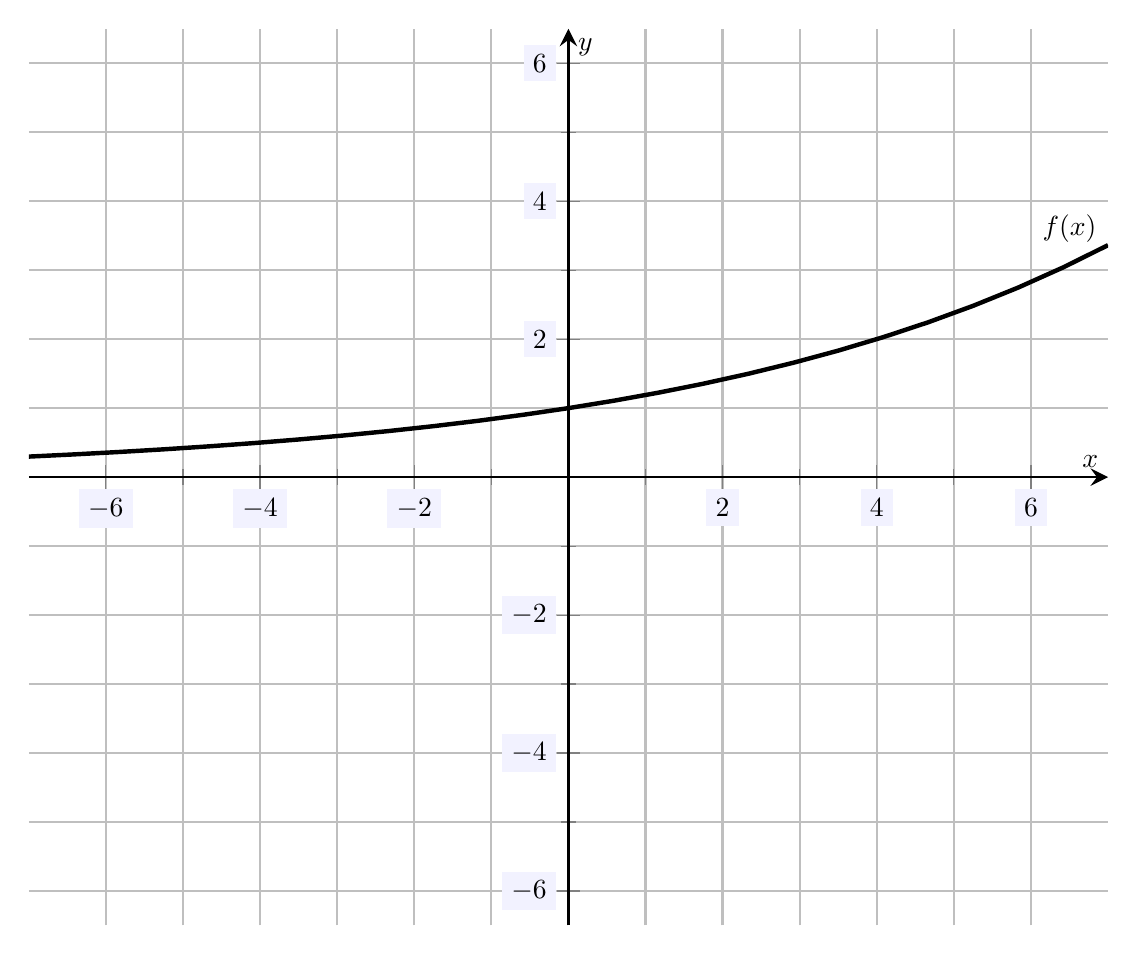
\begin{tikzpicture}[scale=2,every node/.style={scale=0.5}]
	\begin{axis}[
	grid=both,
	axis lines=middle,
	ticklabel style={fill=blue!5!white},
	xmin= -7, xmax=7,
	ymin= -6.5, ymax=6.5,
	xtick={-6,-4,-2,0,2,4,6},
	ytick={-6,-4,-2,0,2,4,6},
	minor tick = {-5,-3,...,5},
	xlabel=\(x\),ylabel=\(y\),
	]
	\node at (6.5,3.6) {$f(x)$};
	\addplot[thick, domain= -7:7] {2^(x/4)};
	\end{axis}
	\end{tikzpicture}
	}
	\] \pspace


\end{document}